The Large Hadron Collider (LHC) is the worlds largest particle collider and the largest physics experiment ever built. 
It comprises, amongst an array of smaller subsystems, a 27km ring around which counter-propagating beams of protons are accelerated to energies of around 6.5 TeV. 
When up to the required energy these proton beams collide head-on at four collision points.
These collision points are:
\begin{itemize}
\item ATLAS and CMS, two general purpose detectors studying Higgs physics and searching for physics beyond the standard model
\item ALICE, studying the quark-gluon plasma that existed moments after the big bang
\item LHCb, investigating the matter-antimatter asymmetry in the universe.
\end{itemize}
The centre of mass energy of the proton-proton ($pp$) collisions is $\sqrt{s}=13$ TeV, where $s$ is the first Mandelstam variable.
Due to the incredibly high energies, very strong magnets are required to guide the proton beams properly.
Around the circumference, there are 1232 superconducting magnets, cooled to 1.9 K generating a magnetic field of 8.33 T.

In order to accelerate the protons to the required energy many smaller sub-accelerators are required, a schematic of which can be seen in figure \ref{fig:LHC}.

\begin{figure}[H] %  figure placement: here, top, bottom, or page
   \centering
   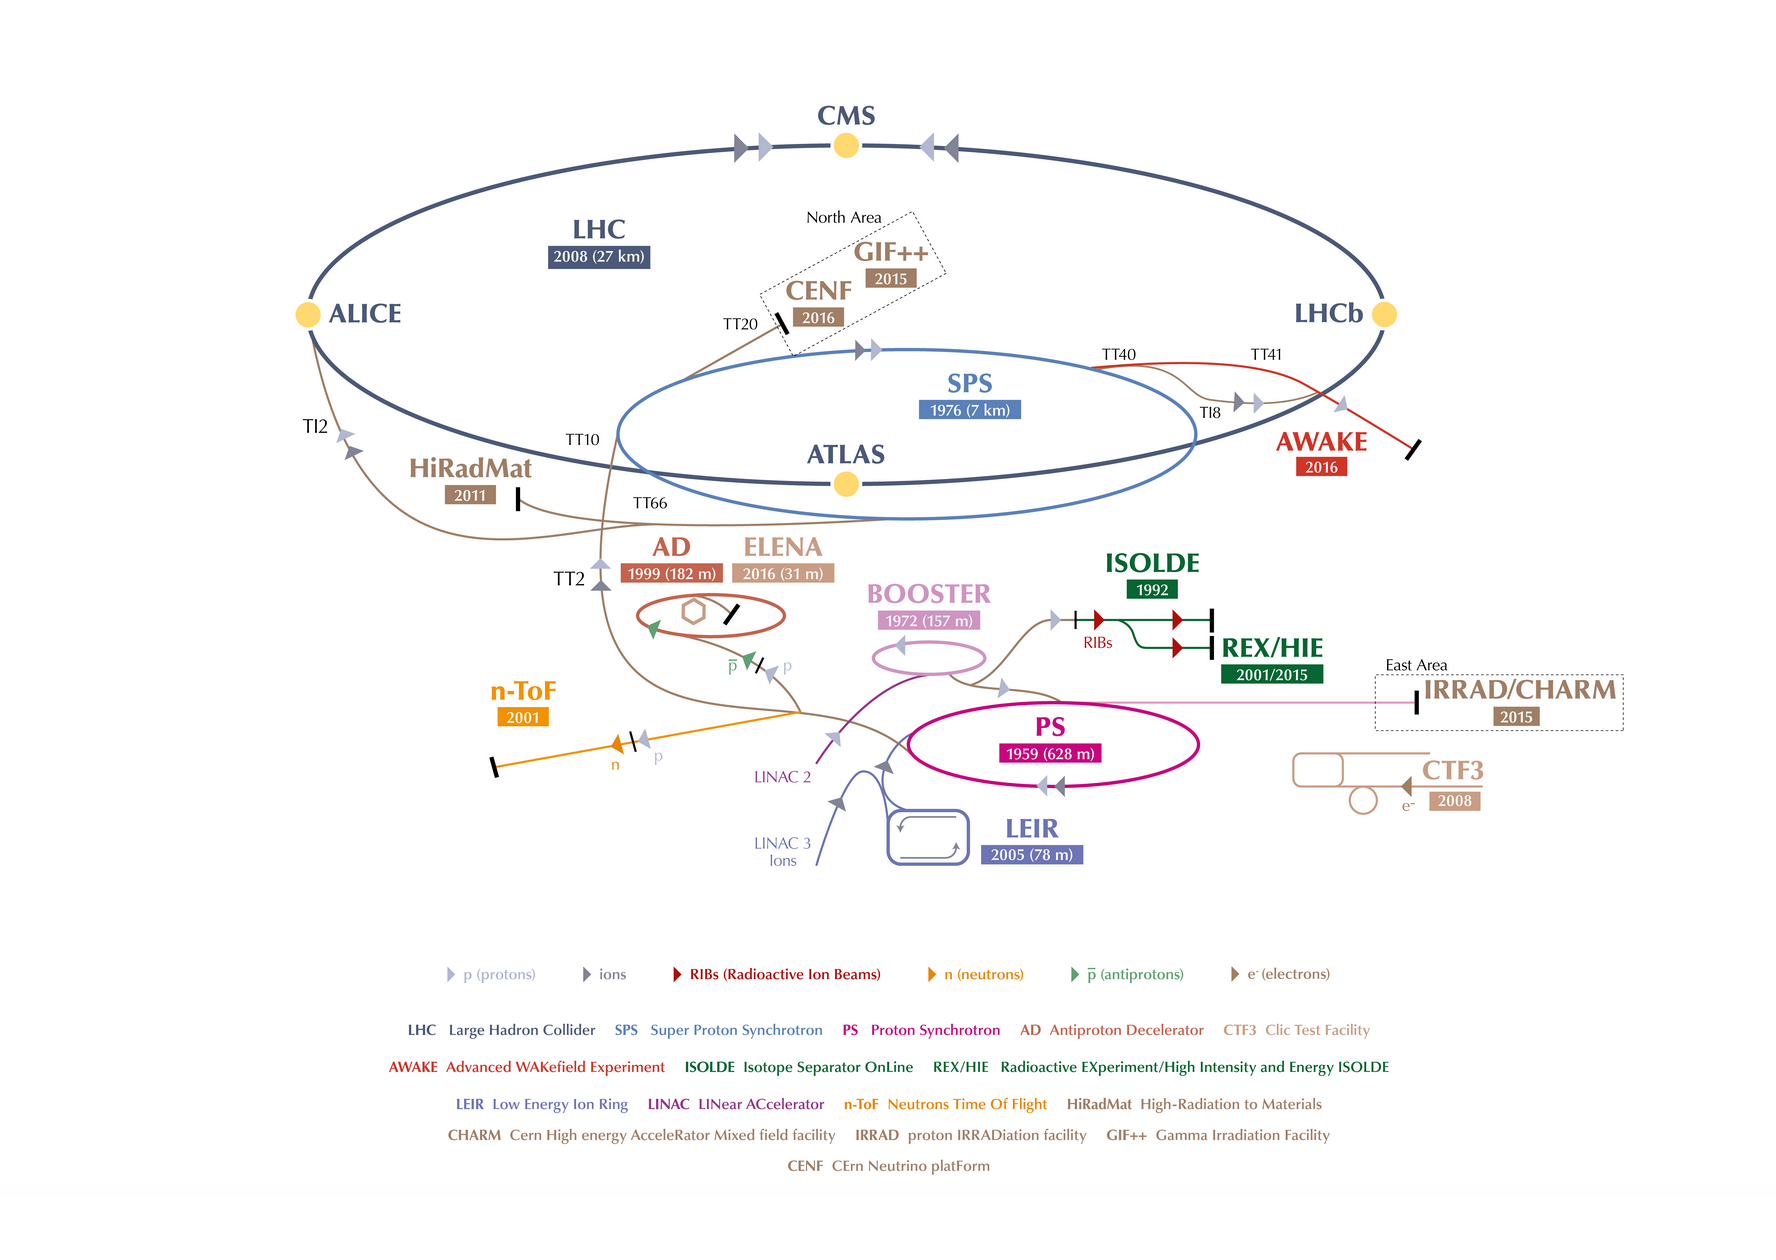
\includegraphics[width=.8\textwidth]{Pictures/LHC.png} 
   \caption{Schematic of the accelerator system at CERN \cite{Mobs:2197559}}
   \label{fig:LHC}
\end{figure}

\noindent The first phase of the acceleration process is the linear accelerator, Linac2. 
Here the protons are initially accelerated to 50 MeV, after which they are injected into the Proton Synchrotron Booster where they are subsequently accelerated to 1.4 GeV.
After this, the protons are sent into the Proton Synchrotron (PS) where they reach an energy of 25 GeV.
The penultimate accelerator the is the Super Proton Synchrotron (SPS) which accelerates the protons to 450 GeV, after which they are injected into the LHC to reach the desired energy of 6.5 TeV.

During this acceleration process, the protons coalesce into `bunches', each containing around 100 billion protons.
One can define the interaction rate of these bunches as

\begin{align}
\frac{d N}{d t} = \sigma \mathcal{L},
\end{align}
where $\sigma$ is the interaction cross-section and $\mathcal{L}$ is the instantaneous luminosity.
One can estimate $dN/dt$, given the proton inelastic cross-section to be about 60 mb, at roughly 1 billion proton interactions per second.
By taking the time integral of the instantaneous luminosity, 
\begin{align}
L = \int \mathcal{L} dt,
\end{align}
one acquires a measure of the number of events collected, the integrated luminosity $L$. 
As technology improves integrated luminosities get larger, furnishing us with the ability to discover rare new processes, such as supersymmetric particle production.

\section{The ATLAS Detector}
The ATLAS detector (\textbf{A} \textbf{T}oroidal \textbf{L}HC \textbf{A}pparatu\textbf{S}) is one of the two multi-purpose detectors at the LHC.
It is 44m long, 25 meters in diameter, and weighs roughly 7000 tonnes making it the largest particle detector ever built.
The purpose of the ATLAS detector is to examine Higgs physics, QCD, and many beyond the Standard Model scenarios.

The ATLAS detector is composed of multiple layers, each of which is responsible for identifying different types of particles. 
The first of these layers is the silicon tracking sensors. 
This is located closest to the beam pipe and is used to determine and reconstruct the trajectories of charged particles passing through it.
A magnetic field of about $2$ T is applied axially across the inner tracking detector, allowing for the determination of charge.
Once the particles leave the tracking detector they first enter the electromagnetic calorimeter.
This is designed to measure the energy of final state photons and electrons by considering the length of their associated showers.
One does not generally observe muon showers in the electromagnetic calorimeter as the muon cross section vastly suppresses its ability to undergo Bremsstrahlung emission.
The penultimate layer is the hadronic calorimeter, designed to detect the hadronic showers from longer-lived hadrons.
Shortly lived hadrons are detected by inference from examining their final state products.
For example, the production of a $\pi^{0}$ meson is inferred by detecting two photons travelling in opposite directions with an invariant mass that allows for the reconstruction of the pion mass. 
Lastly, there is the muon spectrometer designed to detect muons escaping the detector.

A 3D rendering of the detector can be seen in figure \ref{fig:ATLAScrossSection}a and a simplified cross-section of the detector with example particle traces can be seen in figure \ref{fig:ATLAScrossSection}b.
The following subsections will discuss the operation principles of each of the major layers of the ATLAS detector in detail.

\begin{figure}[H]
    \centering
    \begin{subfigure}[b]{0.48\textwidth}
        \centering
        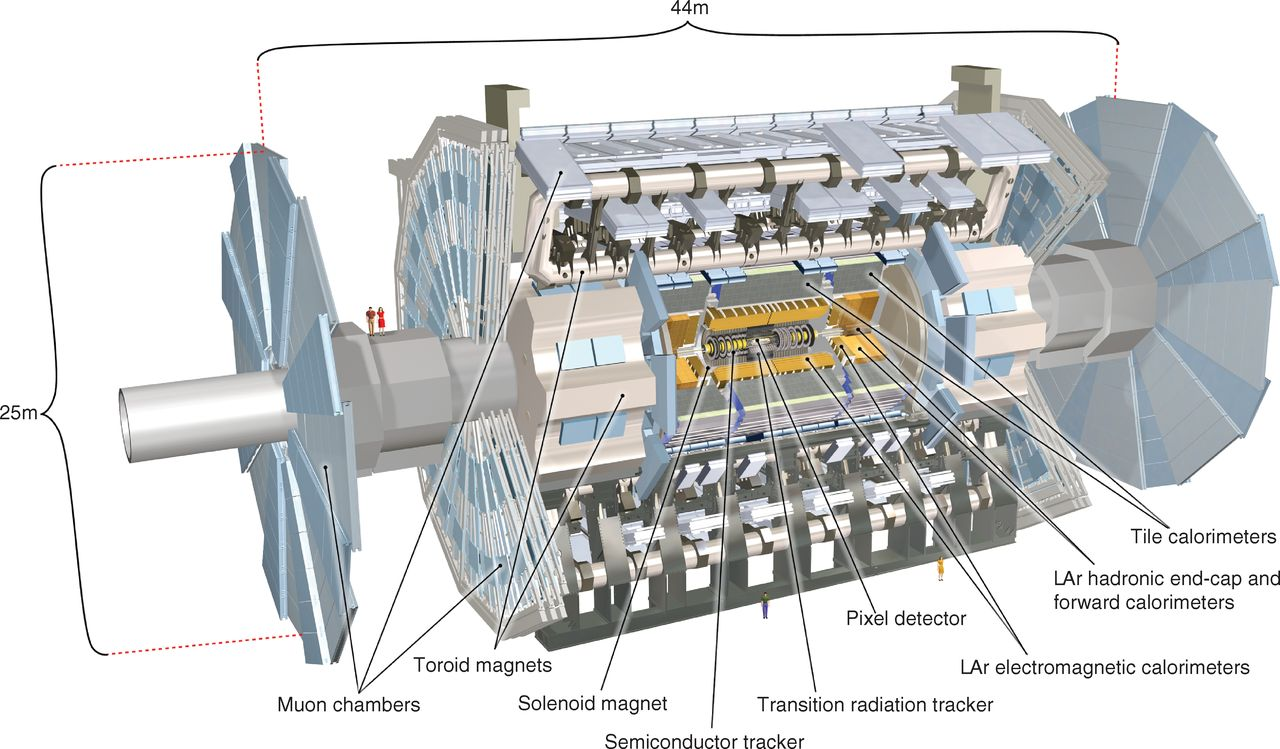
\includegraphics[width=\textwidth]{Pictures/ATLASopen.jpg}
    \caption{}
    \end{subfigure}
    ~
    \begin{subfigure}[b]{0.48\textwidth}
        \centering
        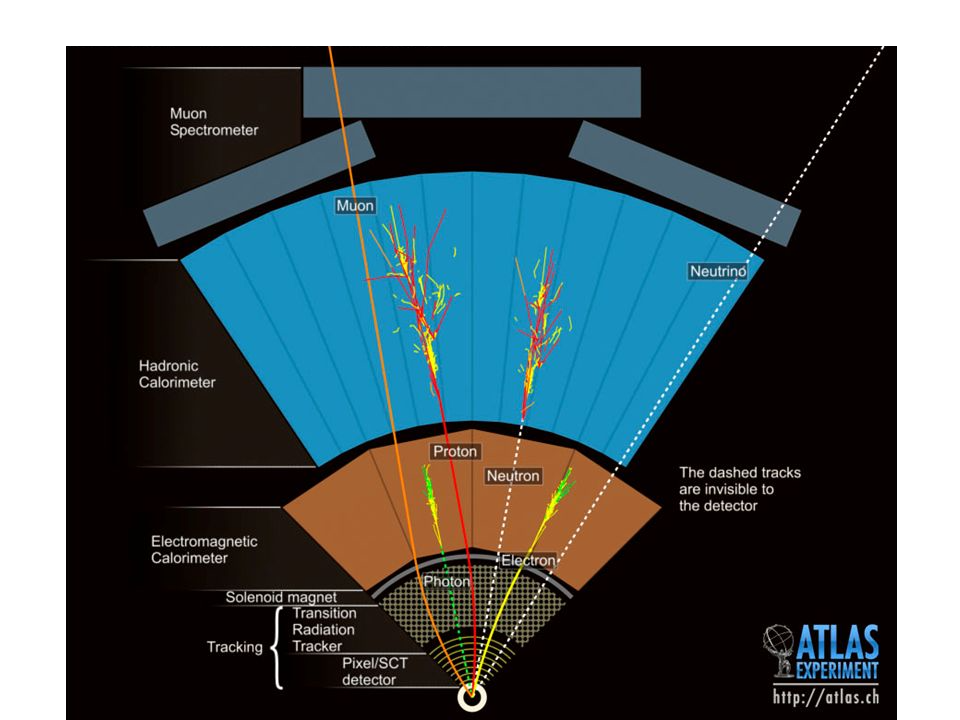
\includegraphics[width=\textwidth]{Pictures/ATLAS-X-sec.png}
    \caption{}    
        \end{subfigure}
\caption{(a) 3D rendering of the ATLAS Detector showing an inside view of the different components \\ (b) Cross section of the ATLAS detector showing example particle traces through the various layers \cite{virdee2012physics}}
\label{fig:ATLAScrossSection}
\end{figure}

\subsection{Co-ordinate Conventions}
In Cartesian co-ordinates one defines the three axes such that $x$ is directed towards the centre of the main LHC ring, $y$ is directly vertical, and $z$ is directed along the beam line.
Generally, because one mostly refers to features of the transverse plane, it is easier to work in polar coordinates such that $\phi=0$ defines the $x$-axis.
One slight difference to conventional polar coordinates is that the angle $\theta$ is replaced with pseudorapidity. 
This is defined as the massless or high energy limit of rapidity, $y$, where
\begin{align}
y = \frac{1}{2} \ln \left( \frac{E + p_{z}}{E - p_{z}} \right).
\end{align}
At high energy one can replace the momentum using
\begin{align}
p_{z} = E \cos \theta. 
\end{align}
Replacing rapidity with pseudorapidity, $\eta$, we get
\begin{align}
\eta = \ln \left( \frac{1 + \cos \theta}{1 - \cos \theta} \right)^{1/2}.
\end{align}
Using half angle trigonometric identities one can show that this is equivalent to
\begin{align}
\eta = - \ln \left( \tan \frac{\theta}{2} \right)
\end{align}
The conversion between angle from the $x$-axis to values of $\eta$ is shown below.

\begin{figure}[H]
    \centering
    \begin{subfigure}[b]{0.48\textwidth}
        \centering
        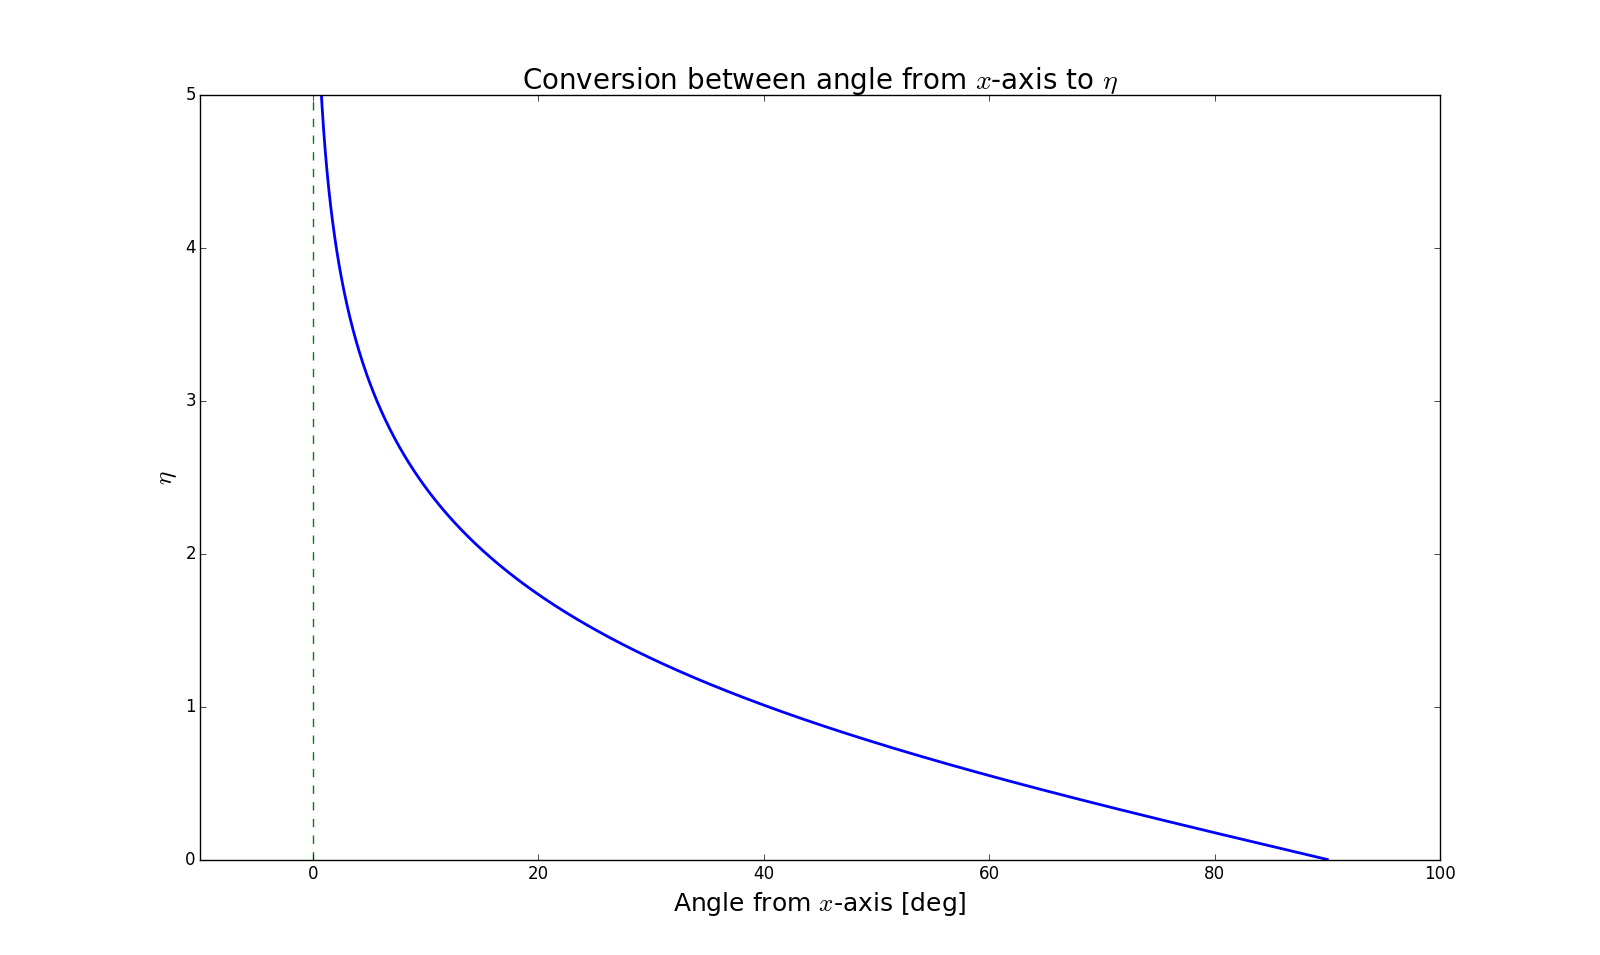
\includegraphics[width=\textwidth]{Pictures/etaConversion.png}
    \caption{}
    \end{subfigure}
    ~
    \begin{subfigure}[b]{0.48\textwidth}
        \centering
        \includegraphics[width=0.7\textwidth]{Pictures/Pseudorapidity2}
    \caption{}    
        \end{subfigure}
\caption{(a) Conversion function of $\eta$ to $\theta$ \\ (b) Pictorial display of the relation between $\eta$ and $\theta$}
\label{fig:etaConversion}
\end{figure}

\subsection{Inner Detector and Tracking}
The innermost component of the ATLAS detector is responsible for particle tracking, referred to as the inner detector (ID).
It is built in layers each consisting of finely segmented detectors allowing for the reconstruction of particle tracks.
It is composed of three main systems: the pixel detector, the semiconductor tracker (SCT), and the transition radiation tracker (TRT); these can be seen in the `Tracking' bracket in figure \ref{fig:ATLAScrossSection}b.
By its construction it is able to cover a solid angle of $\left | \eta \right | < 2.5$.

As stated previously, the inner detector is under a considerable magnetic field. 
This magnetic field, in conjunction with a particle's energy and electric charge, causes curved particle traces.
The inner detector is responsible for quickly identifying these curves paths as from the curvature one can deduce a particle's momentum.

\subsection{Electromagnetic and Hadronic Calorimeters}
The calorimeters measure the energy of the particles interacting with them.
In ATLAS the calorimeters measure the energy of electrons, photons, and hadrons.
As seen in figure \ref{fig:ATLAScrossSection}, ATLAS has an electromagnetic liquid Argon (LAr) calorimeter, and a hadronic calorimeter made of iron scintillator tiles.
Overall, the calorimetry setup covers a solid angle of up to $\left | \eta \right | < 4.9$.
Comparatively the electromagnetic calorimeter provides a more finely grained measurement of electron and photon energies, whereas the hadronic calorimeter is much more coarse in its measurements.
This is not an issue, however, as jet reconstruction can still be achieved as well as measurements of missing transverse energy.

\subsection{Muon Detector}
The muon detectors cover a solid angle of $\left | \eta \right | < 2.7$ and are designed to detect muons by detecting deflection in particle tracks due to magnetic fields.
The magnetic field across the muon detector varies such that the particle track is not one single curve but a combination of many.
At the ATLAS detector, the muon system is used as a trigger to select events with significantly high energy muons and to thereby measure the position of these muons as they travel through the detector.

\subsection{b-jet tagging} \label{subsec:bjetTag}
An important tool in high energy physics is $b$-jet tagging, the process by which jets produced as a result of bottom quark production can be identified.
The tagging of $b$-jets can be done by searching for the signatures of $B$ mesons, mesons that contain bottom quarks.
These mesons are relatively long-lived allowing for them to travel a reasonable distance before ultimately decaying into other particles.
Their lifetimes are not too long, however, allowing for the $B$ mesons to decay within the detector itself. 
With the advent of precision silicon detectors, detectors are able to track the decay products of these $B$ mesons back to the original location of the decay.
One finds that this is not the centre of the interaction, but rather a point displaced by some distance. 
This gives the indication that the jet is a result of a $B$ meson decay.
Additionally, bottom quarks are significantly more massive than their decay products. 
This means that the decay products generally have high transverse momentum, consequently causing $b$-jets to be quite wide with high multiplicities (number of constituent particles).
This is another indicative quality of $b$-jets used in the tagging process.

It is important to note that $b$-jet tagging doesn't have a 100\% success rate.
This means that if one is applying a restriction whereby all events with $b$-jets are discarded, a subset of these events will make it through the selection.

\begin{figure}[H] %  figure placement: here, top, bottom, or page
   \centering
   \includegraphics[width=0.4\textwidth]{Pictures/B-tagging_diagram} 
   \caption{Graphical representation of the identification of $b$-jets}
   \label{fig:bjetTagging}
\end{figure}

\section{Software}
Within the analysis procedure discussed in this dissertation, two main scripts are utilised to achieve two of the most important features of the analysis.
The first framework to be discussed will be the P{\scshape rettyPython} package, developed by Nicola Abraham at the University of Sussex.
This package is responsible for producing the ATLAS style plots of the variables, included extensively in this dissertation.

The second framework used is the Y{\scshape ieldTable} package, developed by the Experimental Particle Physics Group at the University of Sussex.
This package is responsible for determining the resultant counts of each background and signal once subjected to user-defined cuts and conditions.
The output of this program is a table containing a full breakdown of background counts, with associated uncertainties, a combined total with propagated error, and an analogous sample count for each Monte Carlo generated SUSY sample, conveniently formatted into a \LaTeX tabular environment.

\subsection{P{\scshape rettyPython} Framework}
P{\scshape rettyPython} is built as an object-oriented software framework designed to produce histograms of background and signal events. 
In conjunction with the production of histograms, the plots also include a display the yields of the backgrounds and samples, contained within the legend of the plot.
Beneath each histogram produced one has the option of producing a significance trace, showing the relation between the signal and background.
This feature is important, used primarily in this analysis to place contentious cuts on variables related to the sample signals.

\subsubsection{Significance}
A naive approach to significance, relating the quality of the signal with respect to the background, is given as 

\begin{align}
Zn = \frac{S}{\sqrt{B}}, 
\end{align}

\noindent where $S$ and $B$ are the numbers of signal and background yields respectively.
This, however, has its problems, most obviously when the background count is zero $Zn$ goes to infinity.
This would be a non-sensical value for the significance of a given signal.
One solution to this problem is to normalise the significance with respect to the signal yield, as shown below.

\begin{align}
Zn = \frac{S}{S + \sqrt{B}}
\end{align}

\noindent In the analysis procedure, the calculation of significance is done using a more complicated formula, taking into account the fact that the signals and backgrounds in the analysis are estimates, based on a Monte Carlo event generator.
The full formula is defined as \cite{cowan2008discovery}
\begin{align}
Zn = \sqrt{2 \left((S+B)\ln\left(1 + \frac{S}{B} \right) - S\right)}.
\end{align}
\noindent A full breakdown of the derivation of this form of the significance can be found in \cite{cowan2008discovery}.

Conveniently, within the P{\scshape rettyPython} framework the calculation of significance can be processed using the function from the ROOT C++ library: B{\scshape inomialExpZ}.
This function requires three inputs in the format:
\begin{align}
Zn = \texttt{BinomialExpZ}(S_{y}, B_{y}, \sigma_{B, rel})
\end{align}
Where $S$ and $B$ ard the signal and background yields respectively, and $\sigma_{B, rel}$ is the relative background uncertainty, set at $30\%$.
Calculating the significance of a particular sample bin by bin allows for a trace of the significance to be plotted underneath in parallel to the main histogram.
An important consideration to make is that negative overall significance values can be acquired from this method.
These are artefacts of the binomial expansion used in the calculation process and are subsequently interpreted as zero within the analysis.

\subsubsection{Inputs}

In order to have samples and backgrounds in the histograms there exists a class for inputs, defining them as objects with certain properties.
The important parameters that require definition in the construction of the input objects are:
\begin{itemize}
\item the input's name
\item the \texttt{.root} file with the data tree for the particular input
\item the name of the tree within which the data can be found
\item the colour one wants the input to show up as in the final histogram
\item the label for the input as you want it to show up in the legend of the histogram
\item the scaling factor for the data, set to the luminosity of the data ($L = 36.1$ fb$^{-1}$)
\item the weight of the input, defined as a specific combination of values specific to each input.
\end{itemize}

\noindent The constructors for each of the desired inputs are contained with the file \texttt{my\_inputs.py}.
This file is run in conjunction with the main file when producing the plots and determines the specific inputs used in the final histogram.

\subsubsection{Variables}
The variables plotted are themselves objects, constructed using the variable class. 
In order to have stylistic control over the final histogram, one has the ability to define certain properties of the variables.
These include:
\begin{itemize}
\item the variable name as it appears in the \texttt{.root} file
\item the units of this variable, generally this is GeV
\item the label as you want it to appear on the $x$-axis of the histogram
\item the range and number of bins you want in the plot.
\end{itemize}

\noindent The constructors for each of the variables plotted is contained in the file \texttt{my\_vars.py}.
This file is also run in conjunction with the main file when producing plots and defines the particular variables plotted for each of the inputs in a specific histogram.

\subsubsection{Defining signal regions}
Perhaps the most important part of the framework is the environment within which the cuts and limitations are placed on the variables being plotted.
These regions are defined by constructing objects of type 'region'.
There are three main components to the regions used in the analysis discussed in this dissertation.
The first of which is the name of the region, used in the name of the file when created and also printed as a subtitle in the plot.
The second definition to be made is a tuple including all of the cuts that the program must apply when run.
The third definition is another tuple including a list of the 'n minus ones'.
These can be used to add directional arrows showing the position and direction of a cut on a particular variable, or to apply cut on variables whilst plotting a different variable.

Similarly to before, the constructors for the regions are included in the file \texttt{my\_regions\_WZ.py}.
This file is also run in conjunction with the main file, dictating the particular cut combinations applied to the particular variables and inputs in the given histograms.

\subsubsection{Running the software}
Seeing as there are many components required before a plot can be constructed, many files must be run in parallel such that all of the information to make a single plot is available.
Within the package there exists the file \texttt{run.py} containing all of the initiating commands for making the plots.
As previously mentioned, one must run the Python files containing the constructors for the variables, inputs, and regions being used, contained in a directory called \texttt{my\_configurations}.
One can also include the systematics defined analogously to variables and inputs.
Finally, one can apply \texttt{-j n} allowing for the programs to be run on \texttt{n} cores.
This leaves the execution command for the production of variable histograms as shown below.

\begin{center}
\texttt{./run.py -c my\_configurations/my\_inputs.py my\_configurations/my\_vars.py my\_configurations/my\_syst.py my\_configurations/my\_regions\_WZ.py -j n}
\end{center}

\subsection{Y{\scshape ield Table} Framework}

The Y{\scshape ieldTable} framework is responsible for calculating the event yields from each input as well as the associated uncertainty with each yield value.
The output of this is a \texttt{.tex} file with a table of results formatted as a LaTeX tabular environment.

In order to run the script one must define:
\begin{itemize}
\item the directory in which the background and sample \texttt{.root} nTuples are stored
\item the directory in which the data files are stored (these are the official CERN data files, not used in this analysis)
\item a name for the output file, generally in the format \texttt{$<$name$>$.tex}
\item the luminosity used in the analysis, in this case, $L = 36.1$ fb$^{-1}$
\item the label '3L', required to specify the tri-lepton analysis
\item a boolean input of whether or not to analyse the data files.
\end{itemize}

With these primary inputs defined one can go onto to specifying the number of cuts and the combination of conditions within each cut.
The number of cuts applied becomes the number of columns in the final table of results.

Filling the columns once the layout of the table has been made is a relatively simple process.
For each background and sample used a row is defined with the input's name.
The nTuple for the particular input is opened and cycled through, counting all of the entries inside that satisfy the conditions defined in the individual cuts.
Secondly, the uncertainty on the number of events counted is calculated and then written into the output file.
Additionally, a row showing the total combined backgrounds with associated uncertainties for each column are included in the final output.
The outputs of this procedure are referred to as yield tables and will be referred to as such throughout this dissertation.
